\documentclass[10pt]{article}
\usepackage[T1]{fontenc}\usepackage{lmodern}\usepackage[margin=2cm]{geometry}
\usepackage{graphicx,booktabs,longtable,float,xcolor}\usepackage[hidelinks]{hyperref}
\setlength{\parskip}{0.5em}\setlength{\parindent}{0pt}
\definecolor{bp}{HTML}{123A6E}
\begin{document}
{\color{bp}\Large\bfseries RNGD Hotel Floor Plan Optimization: fp1\_multi, Extended Program (3 Levels, 48 Keys)}\par
{\small RNGD design optimizer --- 2026-10-10 22:59 --- site fp1\_multi, program hotel\_program\_extended.json}\par
\fcolorbox{bp}{white}{\parbox{0.96\linewidth}{\small\textbf{AI disclosure.} The prose sections were written by anthropic/claude-sonnet-5.5 from the computed results, grounded with retrieved code passages. All tables and figures come directly from the data. 67 numbers in the AI text were checked against the data: 67 traced.}}

\section{Executive summary}
The optimizer placed all 62 of 62 rooms and all 48 requested keys across three levels on the fp1\_multi site, with a final fitness of 0.9119. The best fitness in the first generation was 0.8972. Daylight, egress, ADA, and corner objectives all scored 1.0, and every exterior-facing check in the data came back at an exterior fraction of 1.0. All six code checks listed in the data pass, including the 50 ft dead-end limit in IBC-R1-027 (provided: 41 ft). The weakest objectives are efficiency (0.6763) and compactness (0.6412), and balance (0.816) is also moderate. The run was short (219 evaluations, 5.6 s) and did not use an LLM review, so the result is a first-pass layout that still needs professional code review.

{\small\begin{longtable}{p{6cm}p{9.5cm}}\toprule
\textbf{Measure} & \textbf{Optimized design} \\ \midrule \endhead
Rooms placed & 62 / 62 \\
Keys placed & 48 / 48 \\
Placed area & 22,831 SF of 22,576 SF \\
Corridor & 936 SF per level (ratio 0.0971) \\
Rooms with a window (where needed) & 1.0 \\
Max exit travel / dead end & 60.1 ft / 40.7 ft \\
Cores reached & 2 / 2 \\
ADA mobility rooms & 5 placed, 2 required \\
Shared walls & 948 ft \\
Fitness & 0.9119 \\
\bottomrule\end{longtable}}

\section{Approach}
Rooms were placed on the fixed site grid with the systematic search method, using a population of 24 for 30 generations (seed 7). The run used 219 evaluations in 5.6 seconds. Fitness is a weighted sum of ten 0-1 objective scores. Placement carries the most weight (0.3), followed by daylight (0.14), egress (0.12), efficiency (0.1), ADA (0.08), core access (0.07), adjacency (0.07), balance (0.05), compactness (0.04), and corner (0.03). No LLM design review was used (use\_llm is false, with 0 checkpoints), so the score reflects only the computed objectives. The best fitness rose from 0.8972 in the first generation to 0.9119 in the last.

\section{Results}
All 62 rooms and all 48 requested keys were placed. The placed area is 22831 sf against a program area of 22576 sf. Corridors take 936 sf, a corridor ratio of 0.0971. Maximum travel is 60.1 ft, the longest dead end is 40.7 ft, and both cores are reached. Daylight scores 1.0, with an exterior fraction of 1.0. Shared wall length is 948 ft. By level: L1 has 20 rooms, 12 keys, and 7820 sf, and also holds the public and back-of-house spaces (lobby/front desk, breakfast/lounge, fitness, luggage, public restrooms, BOH/office). L2 has 22 rooms, 19 keys, and 7827 sf. L3 has 20 rooms, 17 keys, and 7184 sf. The key mix is 7 King, 3 QQ, 1 King Suite, and 1 ADA King on L1. L2 has 10 King, 6 QQ, 1 King Suite, 1 ADA King, and 1 ADA Suite. L3 has 9 King, 5 QQ, 1 King Suite, 1 ADA King, and 1 ADA Suite. Efficiency (0.6763) and compactness (0.6412) are the lowest scores, and balance is 0.816. Core access is 0.8951 and adjacency is 0.9483. The data does not say what drives the lower efficiency and compactness scores.
\begin{figure}[H]\centering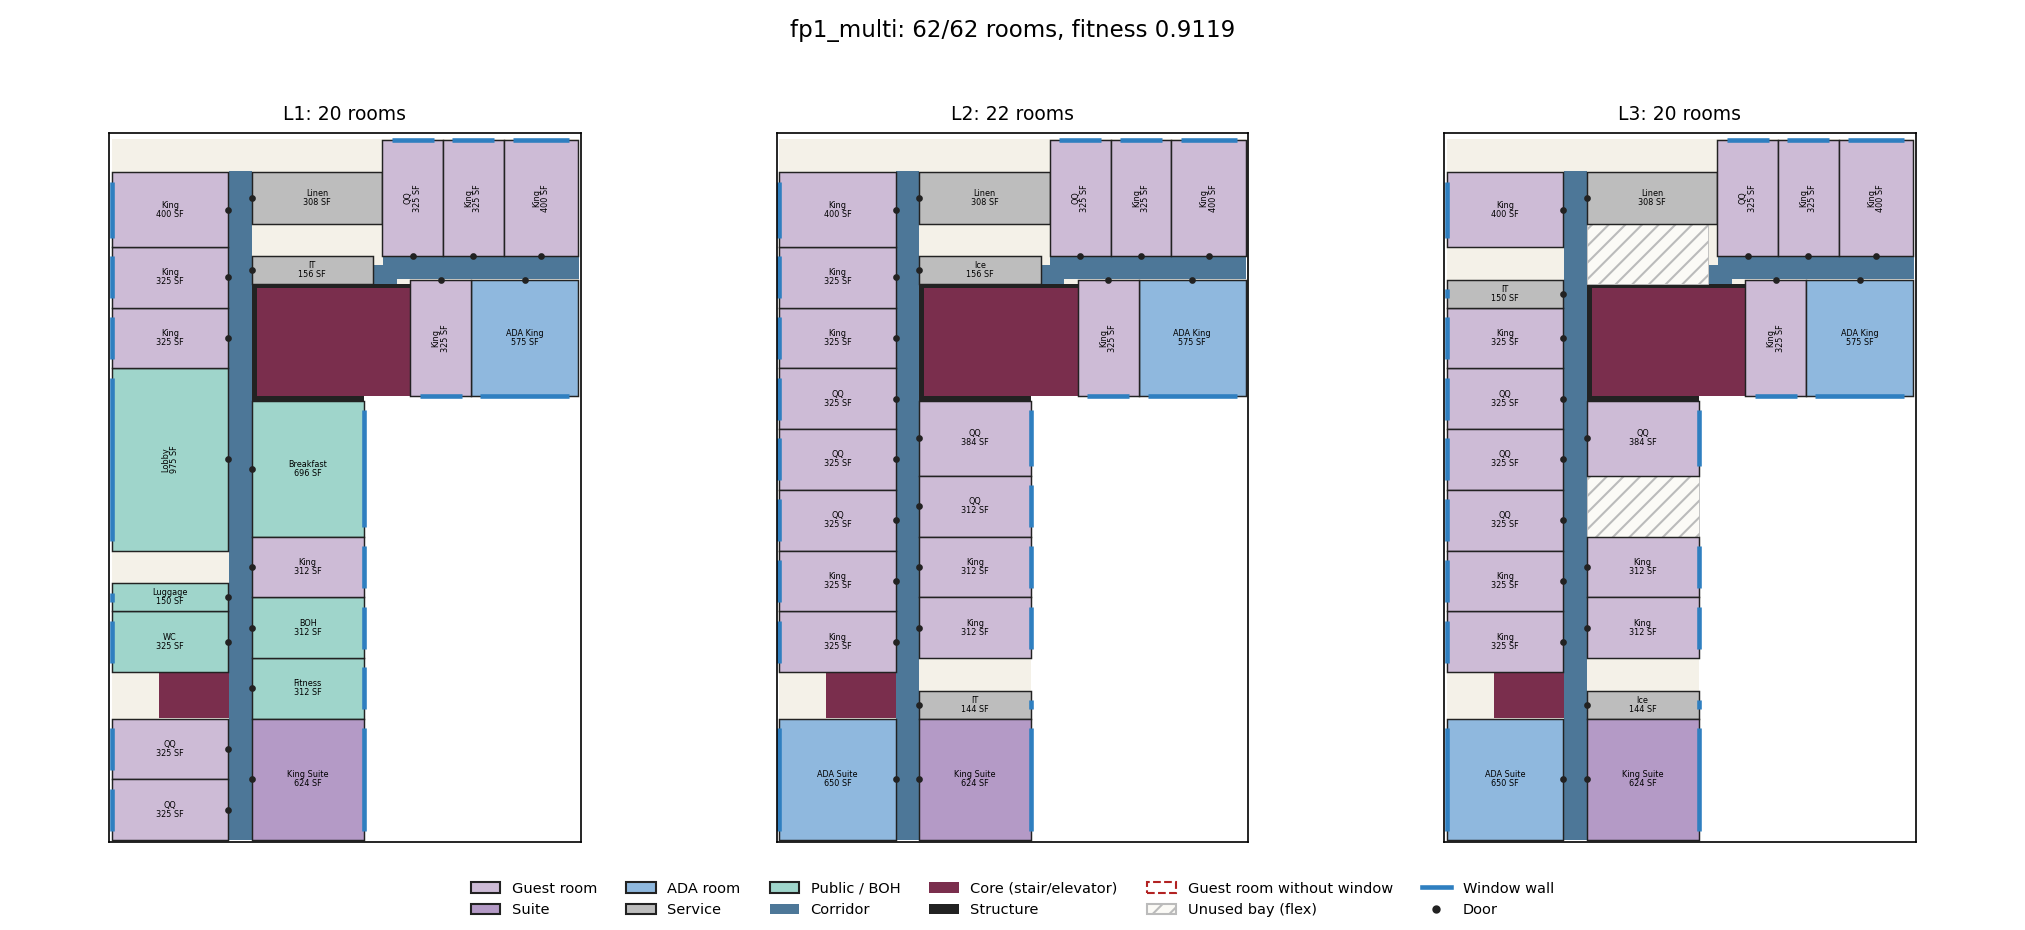
\includegraphics[width=\linewidth]{fp1_multi_plans.png}\caption{Optimized plans, all levels (corridor blue, cores maroon).}\end{figure}
{\small\begin{longtable}{p{1.4cm}p{1.3cm}p{1.2cm}p{1.6cm}p{9.5cm}}\toprule
\textbf{Level} & \textbf{Rooms} & \textbf{Keys} & \textbf{Area SF} & \textbf{Mix} \\ \midrule \endhead
L1 & 20 & 12 & 7,820 & ADA King 1, BOH / Office 1, Breakfast / Lounge 1, Fitness 1, Housekeeping / Linen 1, IT / Elec 1, King 7, King Suite 1, Lobby / Front Desk 1, Luggage 1, Public Restrooms 1, QQ 3 \\
L2 & 22 & 19 & 7,827 & ADA King 1, ADA Suite 1, Housekeeping / Linen 1, IT / Elec 1, Ice / Vending 1, King 10, King Suite 1, QQ 6 \\
L3 & 20 & 17 & 7,184 & ADA King 1, ADA Suite 1, Housekeeping / Linen 1, IT / Elec 1, Ice / Vending 1, King 9, King Suite 1, QQ 5 \\
\bottomrule\end{longtable}}
\begin{figure}[H]\centering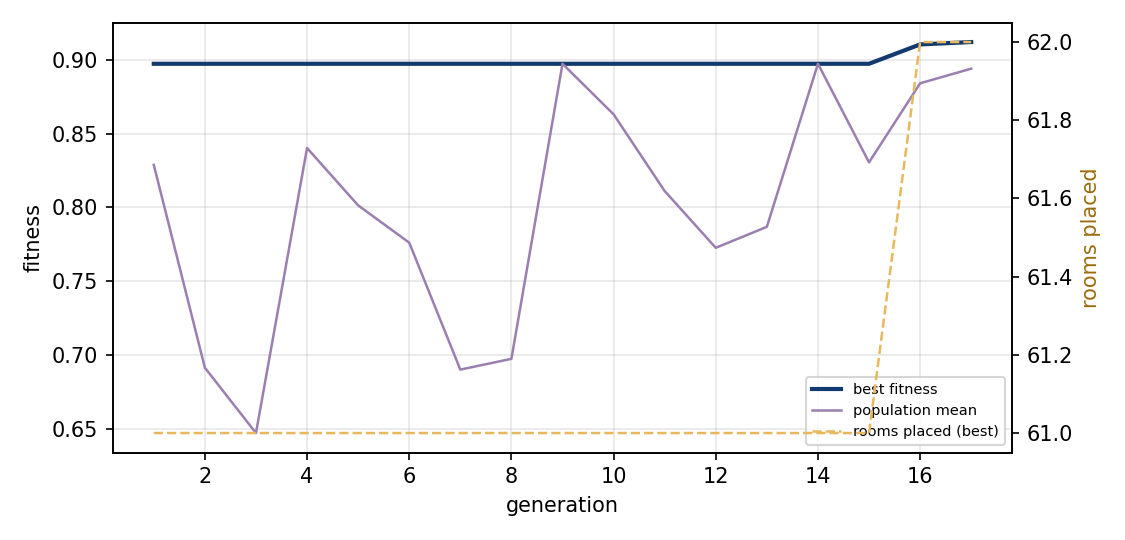
\includegraphics[width=0.85\linewidth]{fp1_multi_convergence.png}\caption{Convergence: best and mean fitness per generation; dotted lines mark LLM reviews.}\end{figure}

\section{Code and accessibility}
All six checks in the data pass. For egress, IBC-R1-015 requires at least 2 exits and 2 are reached. IBC-R1-018 (exit separation) requires 60 ft and the layout provides 81 ft. IBC-R1-023 (exit access travel) allows up to 250 ft and the layout provides 60 ft; the zoning excerpt's stricter 200 ft limit to a stair enclosure would also be met. IBC-R1-025 requires a 44 in corridor and 60 in is provided. IBC-R1-027, the dead-end limit for a fully sprinklered R-1 building, is 50 ft, and the layout provides 41 ft. That rule is marked critical, starter-verified, and requires professional review, so the pass is a screening result and not a code approval. For accessibility, ADA-224.2 is checked at a minimum of 2 mobility rooms for 48 keys, and 5 are provided (one on L1, two each on L2 and L3). They are split between ADA King and ADA Suite types, which is consistent with the dispersion intent of ADA 224.5. The retrieved excerpts do not include the Table 224.2 values, so the required count of 2 comes from the check output and not from the excerpt. The communication-features table (224.4) shown starts at 151 rooms and was not evaluated for this 48-key hotel. IBC-R1-024 requires a 0.5-hour corridor rating, but no check for it appears in the data.
{\small\begin{longtable}{p{1.9cm}p{4.3cm}p{3.6cm}p{3cm}p{1.4cm}}\toprule
\textbf{Rule} & \textbf{Check} & \textbf{Required} & \textbf{Provided} & \textbf{Status} \\ \midrule \endhead
IBC-R1-015 & Exits per story (cores reached) & $\ge$ 2 & 2 & PASS \\
IBC-R1-018 & Exit separation (core to core) & $\ge$ 1/3 diagonal = 60 ft & 81 ft & PASS \\
IBC-R1-023 & Exit access travel & $\le$ 250 ft & 60 ft & PASS \\
IBC-R1-025 & Corridor width & $\ge$ 44 in & 60 in & PASS \\
IBC-R1-027 & Dead-end corridor & $\le$ 50 ft & 41 ft & PASS \\
ADA-224.2 & ADA mobility rooms & $\ge$ 2 for 48 keys & 5 & PASS \\
\bottomrule\end{longtable}}

\section{Comparison with the reference design}\textbf{Note:} the reference was made for the QA program (rooms\_hotel.json) and this design for hotel\_program\_extended.json; room counts are therefore not directly comparable, while the code checks and efficiency measures are.

The reference design (floorplan1.json, 500 generations) reached a fitness of 0.8798 and placed 61 of 72 rooms and 58 keys, with no failed checks. The optimized design reached 0.9119 in 30 generations and placed 62 of 62 rooms and 48 of 48 keys. Its corridor ratio is 0.0971, against 0.1515 for the reference. Its exterior fraction is 1.0, against 0.8793. Its dead end is 40.7 ft, against 47.7 ft. It performs worse on two measures: maximum travel is 60.1 ft against 49.2 ft, and shared wall is 948 ft against 982 ft. The two designs appear to use different programs (62 versus 72 rooms and 48 versus 58 keys), so the fitness values are not a like-for-like comparison. The reference also did not place all of its rooms.

{\small\begin{longtable}{p{5cm}p{5.2cm}p{5.2cm}}\toprule
\textbf{Measure} & \textbf{Reference (floorplan1.json, 500 gens)} & \textbf{Optimized} \\ \midrule \endhead
Rooms placed & 61 & 62 \\
Keys placed & 58 & 48 \\
Fitness (same evaluator) & 0.8798 & 0.9119 \\
Corridor ratio & 0.1515 & 0.0971 \\
Window fraction & 0.8793 & 1.0 \\
Max travel (ft) & 49.2 & 60.1 \\
Dead end (ft) & 47.7 & 40.7 \\
Cores reached & 2 & 2 \\
Shared walls (ft) & 982 & 948 \\
Failed code checks & none & none \\
\bottomrule\end{longtable}}\begin{figure}[H]\centering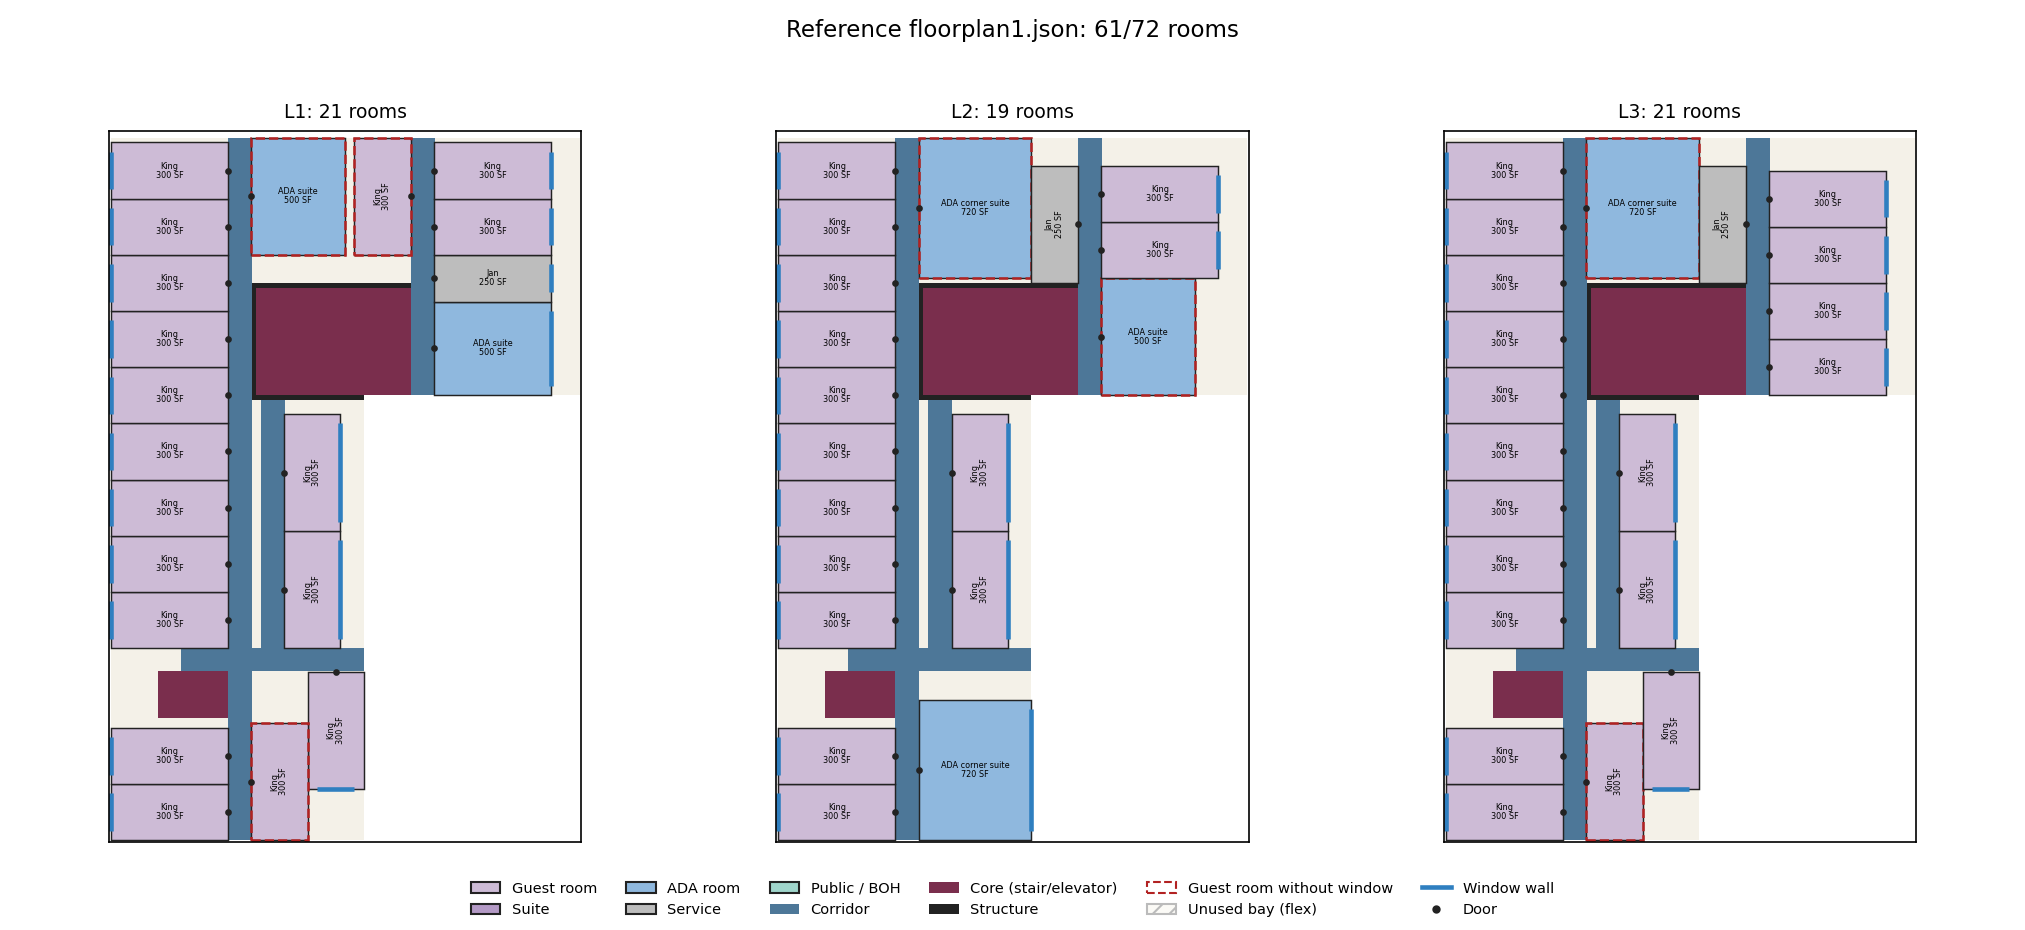
\includegraphics[width=\linewidth]{fp1_multi_reference_plans.png}\caption{Reference design floorplan1.json}\end{figure}

\section{Objectives and weights}
{\small\begin{longtable}{p{2.4cm}p{8.2cm}p{1.6cm}p{2cm}}\toprule
\textbf{Objective} & \textbf{Meaning} & \textbf{Score} & \textbf{Final weight} \\ \midrule \endhead
placement & share of the program placed (priority weighted) & 0.929 & 0.300 \\
daylight & rooms that need a window have an exterior wall & 1.000 & 0.140 \\
efficiency & corridor area kept low & 0.676 & 0.100 \\
egress & exit travel and dead-end corridor within IBC limits & 1.000 & 0.120 \\
ada & ADA mobility rooms: count (Table 224.2) and spread over floors & 1.000 & 0.080 \\
core\_access & service and ADA rooms open close to a core/elevator & 0.895 & 0.070 \\
adjacency & required room adjacencies met & 0.948 & 0.070 \\
corner & suites on corners & 1.000 & 0.030 \\
balance & keys spread evenly over floors & 0.816 & 0.050 \\
compactness & rooms share walls (compact, prefab-friendly) & 0.641 & 0.040 \\
\bottomrule\end{longtable}}

\section{LLM design reviews (inside the fitness function)}
No reviews in this run.

\section{Recommendations}
\begin{itemize}
\item Have a licensed professional review the egress results, especially the critical dead-end rule IBC-R1-027 (41 ft against a 50 ft limit), before the layout is used for permitting.
\item Add checks for corridor fire-resistance rating (IBC-R1-024) and for ADA communication-feature rooms, which the current output does not cover.
\item Run a longer search (more generations or more seeds) and compare the results, since this run used only 30 generations and 219 evaluations.
\item Investigate the low efficiency (0.6763) and compactness (0.6412) scores to see whether the objective weights or the floor geometry cause them.
\item Run the optimization with the LLM design reviewer turned on to get a qualitative check on circulation and room adjacency.
\item Confirm with the developer whether the 48-key program is the intended target, because the reference design had 58 keys.
\end{itemize}

\section{Limitations}
\begin{itemize}
\item Only one search run (seed 7) is reported, so the variability between runs is unknown.
\item No LLM review was used, so the result reflects computed objectives only.
\item Code rules are starter-verified, and the retrieved excerpts mark professional review as required. The pass results are not a compliance determination.
\item The reference design appears to use a different program, so the comparison is indicative only.
\item Some requirements are not modeled or not shown in the data, such as corridor ratings, ADA communication features, and accessible-room details such as bathroom type.
\end{itemize}

\section*{Appendix: fact check of the AI text}
{\small\begin{longtable}{p{4cm}p{5cm}}\toprule
\textbf{Number in text} & \textbf{Result} \\ \midrule \endhead
0.03 & traced to data \\
0.04 & traced to data \\
0.05 & traced to data \\
0.07 & traced to data \\
0.08 & traced to data \\
0.0971 & traced to data \\
0.1 & traced to data \\
0.12 & traced to data \\
0.14 & traced to data \\
0.1515 & traced to data \\
0.3 & traced to data \\
0.5 & traced to data \\
0.6412 & traced to data \\
0.6763 & traced to data \\
0.816 & traced to data \\
0.8793 & traced to data \\
0.8798 & traced to data \\
0.8951 & traced to data \\
0.8972 & traced to data \\
0.9119 & traced to data \\
0.9483 & traced to data \\
1.0 & traced to data \\
12 & traced to data \\
15 & traced to data \\
151 & traced to data \\
17 & traced to data \\
18 & traced to data \\
19 & traced to data \\
20 & traced to data \\
200 & traced to data \\
219 & traced to data \\
22 & traced to data \\
224.2 & traced to data \\
224.4 & traced to data \\
224.5 & traced to data \\
22576 & traced to data \\
22831 & traced to data \\
23 & traced to data \\
24 & traced to data \\
24.2 & traced to data \\
25 & traced to data \\
250 & traced to data \\
27 & traced to data \\
27, & traced to data \\
30 & traced to data \\
40.7 & traced to data \\
41 & traced to data \\
44 & traced to data \\
47.7 & traced to data \\
48 & traced to data \\
49.2 & traced to data \\
5.6 & traced to data \\
50 & traced to data \\
500 & traced to data \\
58 & traced to data \\
60 & traced to data \\
60.1 & traced to data \\
61 & traced to data \\
62 & traced to data \\
7184 & traced to data \\
72 & traced to data \\
7820 & traced to data \\
7827 & traced to data \\
81 & traced to data \\
936 & traced to data \\
948 & traced to data \\
982 & traced to data \\
\bottomrule\end{longtable}}
\end{document}
